\documentclass[journal,12pt,twocolumn]{IEEEtran}
%
\usepackage{setspace}
\usepackage{gensymb}
\usepackage{xcolor}
\usepackage{caption}
%\usepackage{subcaption}
%\doublespacing
\singlespacing

%\usepackage{graphicx}
%\usepackage{amssymb}
%\usepackage{relsize}
\usepackage[cmex10]{amsmath}
\usepackage{mathtools}
%\usepackage{amsthm}
%\interdisplaylinepenalty=2500
%\savesymbol{iint}
%\usepackage{txfonts}
%\restoresymbol{TXF}{iint}
%\usepackage{wasysym}
\usepackage{amsthm}
\usepackage{mathrsfs}
\usepackage{txfonts}
\usepackage{stfloats}
\usepackage{cite}
\usepackage{cases}
\usepackage{mathtools}
\usepackage{subfig}

%\usepackage{xtab}
\usepackage{longtable}
\usepackage{multirow}
%\usepackage{algorithm}
%\usepackage{algpseudocode}
\usepackage{enumitem}
\usepackage{mathtools}
\usepackage{iithtlc}
%\usepackage[framemethod=tikz]{mdframed}
\usepackage{listings}
\usepackage{listings}
    \usepackage[latin1]{inputenc}                                 %%
    \usepackage{color}                                            %%
    \usepackage{array}                                            %%
    \usepackage{longtable}                                        %%
    \usepackage{calc}                                             %%
    \usepackage{multirow}                                         %%
    \usepackage{hhline}                                           %%
    \usepackage{ifthen}                                           %%
  %optionally (for landscape tables embedded in another document): %%
    \usepackage{lscape}     



%\usepackage{stmaryrd}


%\usepackage{wasysym}
%\newcounter{MYtempeqncnt}
\DeclareMathOperator*{\Res}{Res}
%\renewcommand{\baselinestretch}{2}
\renewcommand\thesection{\arabic{section}}
\renewcommand\thesubsection{\thesection.\arabic{subsection}}
\renewcommand\thesubsubsection{\thesubsection.\arabic{subsubsection}}

\renewcommand\thesectiondis{\arabic{section}}
\renewcommand\thesubsectiondis{\thesectiondis.\arabic{subsection}}
\renewcommand\thesubsubsectiondis{\thesubsectiondis.\arabic{subsubsection}}

% correct bad hyphenation here
\hyphenation{op-tical net-works semi-conduc-tor}

%\lstset{
%language=C,
%frame=single, 
%breaklines=true
%}

%\lstset{
	%%basicstyle=\small\ttfamily\bfseries,
	%%numberstyle=\small\ttfamily,
	%language=Octave,
	%backgroundcolor=\color{white},
	%%frame=single,
	%%keywordstyle=\bfseries,
	%%breaklines=true,
	%%showstringspaces=false,
	%%xleftmargin=-10mm,
	%%aboveskip=-1mm,
	%%belowskip=0mm
%}

%\surroundwithmdframed[width=\columnwidth]{lstlisting}
\def\inputGnumericTable{}                                 %%
\lstset{
language=C,
frame=single, 
breaklines=true
}
 

\begin{document}
%

\theoremstyle{definition}
\newtheorem{theorem}{Theorem}[section]
\newtheorem{problem}{Problem}
\newtheorem{proposition}{Proposition}[section]
\newtheorem{lemma}{Lemma}[section]
\newtheorem{corollary}[theorem]{Corollary}
\newtheorem{example}{Example}[section]
\newtheorem{definition}{Definition}[section]
%\newtheorem{algorithm}{Algorithm}[section]
%\newtheorem{cor}{Corollary}
\newcommand{\BEQA}{\begin{eqnarray}}
\newcommand{\EEQA}{\end{eqnarray}}
\newcommand{\define}{\stackrel{\triangle}{=}}

\bibliographystyle{IEEEtran}
%\bibliographystyle{ieeetr}

\providecommand{\nCr}[2]{\,^{#1}C_{#2}} % nCr
\providecommand{\nPr}[2]{\,^{#1}P_{#2}} % nPr
\providecommand{\mbf}{\mathbf}
\providecommand{\pr}[1]{\ensuremath{\Pr\left(#1\right)}}
\providecommand{\qfunc}[1]{\ensuremath{Q\left(#1\right)}}
\providecommand{\sbrak}[1]{\ensuremath{{}\left[#1\right]}}
\providecommand{\lsbrak}[1]{\ensuremath{{}\left[#1\right.}}
\providecommand{\rsbrak}[1]{\ensuremath{{}\left.#1\right]}}
\providecommand{\brak}[1]{\ensuremath{\left(#1\right)}}
\providecommand{\lbrak}[1]{\ensuremath{\left(#1\right.}}
\providecommand{\rbrak}[1]{\ensuremath{\left.#1\right)}}
\providecommand{\cbrak}[1]{\ensuremath{\left\{#1\right\}}}
\providecommand{\lcbrak}[1]{\ensuremath{\left\{#1\right.}}
\providecommand{\rcbrak}[1]{\ensuremath{\left.#1\right\}}}
\theoremstyle{remark}
\newtheorem{rem}{Remark}
\newcommand{\sgn}{\mathop{\mathrm{sgn}}}
\providecommand{\abs}[1]{\left\vert#1\right\vert}
\providecommand{\res}[1]{\Res\displaylimits_{#1}} 
\providecommand{\norm}[1]{\lVert#1\rVert}
\providecommand{\mtx}[1]{\mathbf{#1}}
\providecommand{\mean}[1]{E\left[ #1 \right]}
\providecommand{\fourier}{\overset{\mathcal{F}}{ \rightleftharpoons}}
%\providecommand{\hilbert}{\overset{\mathcal{H}}{ \rightleftharpoons}}
\providecommand{\system}{\overset{\mathcal{H}}{ \longleftrightarrow}}
	%\newcommand{\solution}[2]{\textbf{Solution:}{#1}}
\newcommand{\solution}{\noindent \textbf{Solution: }}
\providecommand{\dec}[2]{\ensuremath{\overset{#1}{\underset{#2}{\gtrless}}}}
\DeclarePairedDelimiter{\ceil}{\lceil}{\rceil}
\makeatletter
\@addtoreset{figure}{problem}
\makeatother

%\numberwithin{equation}{subsection}
\numberwithin{equation}{problem}
%\numberwithin{problem}{subsection}
%\numberwithin{definition}{subsection}
\makeatletter
\@addtoreset{figure}{problem}
\makeatother

\let\StandardTheFigure\thefigure
%\renewcommand{\thefigure}{\theproblem.\arabic{figure}}
\renewcommand{\thefigure}{\theproblem}


%\numberwithin{figure}{subsection}

%\numberwithin{equation}{subsection}
%\numberwithin{equation}{section}
\numberwithin{equation}{problem}
%\numberwithin{problem}{subsection}
\numberwithin{problem}{section}
%%\numberwithin{definition}{subsection}
%\makeatletter
%\@addtoreset{figure}{problem}
%\makeatother
\makeatletter
\@addtoreset{table}{problem}
\makeatother

\let\StandardTheFigure\thefigure
\let\StandardTheTable\thetable
%%\renewcommand{\thefigure}{\theproblem.\arabic{figure}}
%\renewcommand{\thefigure}{\theproblem}

%%\numberwithin{figure}{section}

%%\numberwithin{figure}{subsection}



\def\putbox#1#2#3{\makebox[0in][l]{\makebox[#1][l]{}\raisebox{\baselineskip}[0in][0in]{\raisebox{#2}[0in][0in]{#3}}}}
     \def\rightbox#1{\makebox[0in][r]{#1}}
     \def\centbox#1{\makebox[0in]{#1}}
     \def\topbox#1{\raisebox{-\baselineskip}[0in][0in]{#1}}
     \def\midbox#1{\raisebox{-0.5\baselineskip}[0in][0in]{#1}}

\vspace{3cm}

\title{ 
	\logo{
Digital IIR Filter Design
	}
}



% paper title
% can use linebreaks \\ within to get better formatting as desired
%\title{Digital Band Pass Filter design}
%
%
% author names and IEEE memberships
% note positions of commas and nonbreaking spaces ( ~ ) LaTeX will not break
% a structure at a ~ so this keeps an author's name from being broken across
% two lines.
% use \thanks{} to gain access to the first footnote area
% a separate \thanks must be used for each paragraph as LaTeX2e's \thanks
% was not built to handle multiple paragraphs
%

\author{Hemanth Kumar Desineedi and G V V Sharma$^{*}$% <-this % stops a space
\thanks{*The author is with the Department
of Electrical Engineering, Indian Institute of Technology, Hyderabad
502285 India e-mail:  gadepall@iith.ac.in. All content in this manual is released under GNU GPL.  Free and open source.}% <-this % stops a space
%\thanks{J. Doe and J. Doe are with Anonymous University.}% <-this % stops a space
%\thanks{Manuscript received April 19, 2005; revised January 11, 2007.}}
}
% note the % following the last \IEEEmembership and also \thanks - 
% these prevent an unwanted space from occurring between the last author name
% and the end of the author line. i.e., if you had this:
% 
% \author{....lastname \thanks{...} \thanks{...} }
%                     ^------------^------------^----Do not want these spaces!
%
% a space would be appended to the last name and could cause every name on that
% line to be shifted left slightly. This is one of those "LaTeX things". For
% instance, "\textbf{A} \textbf{B}" will typeset as "A B" not "AB". To get
% "AB" then you have to do: "\textbf{A}\textbf{B}"
% \thanks is no different in this regard, so shield the last } of each \thanks
% that ends a line with a % and do not let a space in before the next \thanks.
% Spaces after \IEEEmembership other than the last one are OK (and needed) as
% you are supposed to have spaces between the names. For what it is worth,
% this is a minor point as most people would not even notice if the said evil
% space somehow managed to creep in.



% The paper headers
%\markboth{Journal of \LaTeX\ Class Files,~Vol.~6, No.~1, January~2007}%
%{Shell \MakeLowercase{\textit{et al.}}: Bare Demo of IEEEtran.cls for Journals}
% The only time the second header will appear is for the odd numbered pages
% after the title page when using the twoside option.
% 
% *** Note that you probably will NOT want to include the author's ***
% *** name in the headers of peer review papers.                   ***
% You can use \ifCLASSOPTIONpeerreview for conditional compilation here if
% you desire.




% If you want to put a publisher's ID mark on the page you can do it like
% this:
%\IEEEpubid{0000--0000/00\$00.00~\copyright~2007 IEEE}
% Remember, if you use this you must call \IEEEpubidadjcol in the second
% column for its text to clear the IEEEpubid mark.



% make the title area
\maketitle

\tableofcontents

\bigskip

\begin{abstract}
%\boldmath
The process of designing analog and digital filters is explained by designing a band-pass filter. IIR LPF,BPF filters are designed. All computations are
done in Python. The Chebychev function is employed for designing the IIR filter.
% and the Kaiser window is used for the FIR filter.
\end{abstract}
% IEEEtran.cls defaults to using nonbold math in the Abstract.
% This preserves the distinction between vectors and scalars. However,
% if the journal you are submitting to favors bold math in the abstract,
% then you can use LaTeX's standard command \boldmath at the very start
% of the abstract to achieve this. Many IEEE journals frown on math
% in the abstract anyway.

% Note that keywords are not normally used for peerreview papers.
%\begin{IEEEkeywords}
%Cooperative diversity, decode and forward, piecewise linear
%\end{IEEEkeywords}



% For peer review papers, you can put extra information on the cover
% page as needed:
% \ifCLASSOPTIONpeerreview
% \begin{center} \bfseries EDICS Category: 3-BBND \end{center}
% \fi
%
% For peerreview papers, this IEEEtran command inserts a page break and
% creates the second title. It will be ignored for other modes.
\IEEEpeerreviewmaketitle


%\newpage
%\section{Component Pin Diagrams}
%%
%\input{chapter1}
%

%\newpage

\section{Analog Filter Specifications}
The filter specifications are available in Table \ref{table:specs}.
%%%%%%%%%%%%%%%%%%%%%%%%%%%%%%%%%%%%%%%%%%%%%%%%%%%%%%%%%%%%%%%%%%%%%%
%%                                                                  %%
%%  This is the header of a LaTeX2e file exported from Gnumeric.    %%
%%                                                                  %%
%%  This file can be compiled as it stands or included in another   %%
%%  LaTeX document. The table is based on the longtable package so  %%
%%  the longtable options (headers, footers...) can be set in the   %%
%%  preamble section below (see PRAMBLE).                           %%
%%                                                                  %%
%%  To include the file in another, the following two lines must be %%
%%  in the including file:                                          %%
%%        \def\inputGnumericTable{}                                 %%
%%  at the beginning of the file and:                               %%
%%        \input{name-of-this-file.tex}                             %%
%%  where the table is to be placed. Note also that the including   %%
%%  file must use the following packages for the table to be        %%
%%  rendered correctly:                                             %%
%%    \usepackage[latin1]{inputenc}                                 %%
%%    \usepackage{color}                                            %%
%%    \usepackage{array}                                            %%
%%    \usepackage{longtable}                                        %%
%%    \usepackage{calc}                                             %%
%%    \usepackage{multirow}                                         %%
%%    \usepackage{hhline}                                           %%
%%    \usepackage{ifthen}                                           %%
%%  optionally (for landscape tables embedded in another document): %%
%%    \usepackage{lscape}                                           %%
%%                                                                  %%
%%%%%%%%%%%%%%%%%%%%%%%%%%%%%%%%%%%%%%%%%%%%%%%%%%%%%%%%%%%%%%%%%%%%%%



%%  This section checks if we are begin input into another file or  %%
%%  the file will be compiled alone. First use a macro taken from   %%
%%  the TeXbook ex 7.7 (suggestion of Han-Wen Nienhuys).            %%
\def\ifundefined#1{\expandafter\ifx\csname#1\endcsname\relax}


%%  Check for the \def token for inputed files. If it is not        %%
%%  defined, the file will be processed as a standalone and the     %%
%%  preamble will be used.                                          %%
\ifundefined{inputGnumericTable}

%%  We must be able to close or not the document at the end.        %%
	\def\gnumericTableEnd{\end{document}}


%%%%%%%%%%%%%%%%%%%%%%%%%%%%%%%%%%%%%%%%%%%%%%%%%%%%%%%%%%%%%%%%%%%%%%
%%                                                                  %%
%%  This is the PREAMBLE. Change these values to get the right      %%
%%  paper size and other niceties.                                  %%
%%                                                                  %%
%%%%%%%%%%%%%%%%%%%%%%%%%%%%%%%%%%%%%%%%%%%%%%%%%%%%%%%%%%%%%%%%%%%%%%

	\documentclass[12pt%
			  %,landscape%
                    ]{report}
       \usepackage[latin1]{inputenc}
       \usepackage{fullpage}
       \usepackage{color}
       \usepackage{array}
       \usepackage{longtable}
       \usepackage{calc}
       \usepackage{multirow}
       \usepackage{hhline}
       \usepackage{ifthen}

	\begin{document}


%%  End of the preamble for the standalone. The next section is for %%
%%  documents which are included into other LaTeX2e files.          %%
\else

%%  We are not a stand alone document. For a regular table, we will %%
%%  have no preamble and only define the closing to mean nothing.   %%
    \def\gnumericTableEnd{}

%%  If we want landscape mode in an embedded document, comment out  %%
%%  the line above and uncomment the two below. The table will      %%
%%  begin on a new page and run in landscape mode.                  %%
%       \def\gnumericTableEnd{\end{landscape}}
%       \begin{landscape}


%%  End of the else clause for this file being \input.              %%
\fi

%%%%%%%%%%%%%%%%%%%%%%%%%%%%%%%%%%%%%%%%%%%%%%%%%%%%%%%%%%%%%%%%%%%%%%
%%                                                                  %%
%%  The rest is the gnumeric table, except for the closing          %%
%%  statement. Changes below will alter the table's appearance.     %%
%%                                                                  %%
%%%%%%%%%%%%%%%%%%%%%%%%%%%%%%%%%%%%%%%%%%%%%%%%%%%%%%%%%%%%%%%%%%%%%%

\providecommand{\gnumericmathit}[1]{#1} 
%%  Uncomment the next line if you would like your numbers to be in %%
%%  italics if they are italizised in the gnumeric table.           %%
%\renewcommand{\gnumericmathit}[1]{\mathit{#1}}
\providecommand{\gnumericPB}[1]%
{\let\gnumericTemp=\\#1\let\\=\gnumericTemp\hspace{0pt}}
 \ifundefined{gnumericTableWidthDefined}
        \newlength{\gnumericTableWidth}
        \newlength{\gnumericTableWidthComplete}
        \newlength{\gnumericMultiRowLength}
        \global\def\gnumericTableWidthDefined{}
 \fi
%% The following setting protects this code from babel shorthands.  %%
 \ifthenelse{\isundefined{\languageshorthands}}{}{\languageshorthands{english}}
%%  The default table format retains the relative column widths of  %%
%%  gnumeric. They can easily be changed to c, r or l. In that case %%
%%  you may want to comment out the next line and uncomment the one %%
%%  thereafter                                                      %%
\providecommand\gnumbox{\makebox[0pt]}
%%\providecommand\gnumbox[1][]{\makebox}

%% to adjust positions in multirow situations                       %%
\setlength{\bigstrutjot}{\jot}
\setlength{\extrarowheight}{\doublerulesep}

%%  The \setlongtables command keeps column widths the same across  %%
%%  pages. Simply comment out next line for varying column widths.  %%
\setlongtables

\setlength\gnumericTableWidth{%
	162pt+%
	51pt+%
	38pt+%
0pt}
\def\gumericNumCols{3}
\setlength\gnumericTableWidthComplete{\gnumericTableWidth+%
         \tabcolsep*\gumericNumCols*2+\arrayrulewidth*\gumericNumCols}
\ifthenelse{\lengthtest{\gnumericTableWidthComplete > \linewidth}}%
         {\def\gnumericScale{\ratio{\linewidth-%
                        \tabcolsep*\gumericNumCols*2-%
                        \arrayrulewidth*\gumericNumCols}%
{\gnumericTableWidth}}}%
{\def\gnumericScale{1}}

%%%%%%%%%%%%%%%%%%%%%%%%%%%%%%%%%%%%%%%%%%%%%%%%%%%%%%%%%%%%%%%%%%%%%%
%%                                                                  %%
%% The following are the widths of the various columns. We are      %%
%% defining them here because then they are easier to change.       %%
%% Depending on the cell formats we may use them more than once.    %%
%%                                                                  %%
%%%%%%%%%%%%%%%%%%%%%%%%%%%%%%%%%%%%%%%%%%%%%%%%%%%%%%%%%%%%%%%%%%%%%%

\ifthenelse{\isundefined{\gnumericColA}}{\newlength{\gnumericColA}}{}\settowidth{\gnumericColA}{\begin{tabular}{@{}p{162pt*\gnumericScale}@{}}x\end{tabular}}
\ifthenelse{\isundefined{\gnumericColB}}{\newlength{\gnumericColB}}{}\settowidth{\gnumericColB}{\begin{tabular}{@{}p{51pt*\gnumericScale}@{}}x\end{tabular}}
\ifthenelse{\isundefined{\gnumericColC}}{\newlength{\gnumericColC}}{}\settowidth{\gnumericColC}{\begin{tabular}{@{}p{38pt*\gnumericScale}@{}}x\end{tabular}}

\begin{table}[!h]
\begin{tabular}[c]{%
	b{\gnumericColA}%
	b{\gnumericColB}%
	b{\gnumericColC}%
	}

%%%%%%%%%%%%%%%%%%%%%%%%%%%%%%%%%%%%%%%%%%%%%%%%%%%%%%%%%%%%%%%%%%%%%%
%%  The longtable options. (Caption, headers... see Goosens, p.124) %%
%	\caption{The Table Caption.}             \\	%
% \hline	% Across the top of the table.
%%  The rest of these options are table rows which are placed on    %%
%%  the first, last or every page. Use \multicolumn if you want.    %%

%%  Header for the first page.                                      %%
%	\multicolumn{3}{c}{The First Header} \\ \hline 
%	\multicolumn{1}{c}{colTag}	%Column 1
%	&\multicolumn{1}{c}{colTag}	%Column 2
%	&\multicolumn{1}{c}{colTag}	\\ \hline %Last column
%	\endfirsthead

%%  The running header definition.                                  %%
%	\hline
%	\multicolumn{3}{l}{\ldots\small\slshape continued} \\ \hline
%	\multicolumn{1}{c}{colTag}	%Column 1
%	&\multicolumn{1}{c}{colTag}	%Column 2
%	&\multicolumn{1}{c}{colTag}	\\ \hline %Last column
%	\endhead

%%  The running footer definition.                                  %%
%	\hline
%	\multicolumn{3}{r}{\small\slshape continued\ldots} \\
%	\endfoot

%%  The ending footer definition.                                   %%
%	\multicolumn{3}{c}{That's all folks} \\ \hline 
%	\endlastfoot
%%%%%%%%%%%%%%%%%%%%%%%%%%%%%%%%%%%%%%%%%%%%%%%%%%%%%%%%%%%%%%%%%%%%%%

\hhline{|-|-|-}
	 \multicolumn{1}{|p{\gnumericColA}|}%
	{\gnumericPB{\raggedright}\textbf{Item}}
	&\multicolumn{1}{p{\gnumericColB}|}%
	{\gnumericPB{\raggedright}\textbf{Symbol}}
	&\multicolumn{1}{p{\gnumericColC}|}%
	{\gnumericPB{\raggedright}\textbf{Value}}
\\
\hhline{|---|}
	 \multicolumn{1}{|p{\gnumericColA}|}%
	{\gnumericPB{\raggedright}Sampling Rate}
	&\multicolumn{1}{p{\gnumericColB}|}%
	{$F_s$}
	&\multicolumn{1}{p{\gnumericColC}|}%
	{48 kHz}
\\
\hhline{|---|}
	 \multicolumn{1}{|p{\gnumericColA}|}%
	{\gnumericPB{\raggedright}Pass Band Tolerance}
	&\multicolumn{1}{p{\gnumericColB}|}%
	{$\delta_1$}
	&\multicolumn{1}{p{\gnumericColC}|}%
	{0.15}
\\
\hhline{|---|}
	 \multicolumn{1}{|p{\gnumericColA}|}%
	{\gnumericPB{\raggedright}Stop Band Tolerance}
	&\multicolumn{1}{p{\gnumericColB}|}%
	{$\delta_2$}
	&\multicolumn{1}{p{\gnumericColC}|}%
	{0.15}
\\
\hhline{|---|}
	 \multicolumn{1}{|p{\gnumericColA}|}%
	{\gnumericPB{\raggedright}Passband Lower Cutoff Frequency}
	&\multicolumn{1}{p{\gnumericColB}|}%
	{$F_{p2}$}
	&\multicolumn{1}{p{\gnumericColC}|}%
	{6 kHz}
\\
\hhline{|---|}
	 \multicolumn{1}{|p{\gnumericColA}|}%
	{\gnumericPB{\raggedright}Passband Higher Cutoff Frequency}
	&\multicolumn{1}{p{\gnumericColB}|}%
	{$F_{p1}$}
	&\multicolumn{1}{p{\gnumericColC}|}%
	{7.2 kHz}
\\
\hhline{|---|}
	 \multicolumn{1}{|p{\gnumericColA}|}%
	{\gnumericPB{\raggedright}Transition Band}
	&\multicolumn{1}{p{\gnumericColB}|}%
	{$\Delta F$}
	&\multicolumn{1}{p{\gnumericColC}|}%
	{0.3 kHz}
\\
\hhline{|---|}
	 \multicolumn{1}{|p{\gnumericColA}|}%
	{\gnumericPB{\raggedright}Stopband Lower Cutoff Frequency}
	&\multicolumn{1}{p{\gnumericColB}|}%
	{$F_{s2}$}
	&\multicolumn{1}{p{\gnumericColC}|}%
	{5.7 kHz}
\\
\hhline{|---|}
	 \multicolumn{1}{|p{\gnumericColA}|}%
	{\gnumericPB{\raggedright}Stopband Higher Cutoff Frequency}
	&\multicolumn{1}{p{\gnumericColB}|}%
	{$F_{s1}$}
	&\multicolumn{1}{p{\gnumericColC}|}%
	{7.5 kHz}
\\
\hhline{|-|-|-|}
\end{tabular}
\caption{}
\label{table:specs}
\end{table}


\ifthenelse{\isundefined{\languageshorthands}}{}{\languageshorthands{\languagename}}
\gnumericTableEnd

\renewcommand{\thetable}{\theproblem}
%\begin{enumerate}
%
%\item Sampling rate(\textit{F$_s$})=48 kHz
%
%\item Pass band tolerance($\delta_1$) and stop band tolerance($\delta_2$) are equal.
% 
% i.e. $\delta_1$=$\delta_2$=$\delta$=0.15
% 
%\item Filter pass band range is 6 kHz-7.2 kHz.
%
% i.e. (\textit{F$_{p1}$})=7.2 kHz and (\textit{F$_{p2}$})=6 kHz
%\item Transition band ($\Delta\textit{F}$)= 0.3 kHz. Hence filter stop band range is 5.7 kHz-7.5 kHz.
%
% i.e. (\textit{F$_{s1}$})=7.5 kHz and (\textit{F$_{s2}$})=5.7 kHz
%\end{enumerate}
\section{Digital Filter Specification}
\subsection{Bilinear Tranformation}
\begin{problem}
Obtain the fiter specifications in the $\omega$ domain.
\end{problem}
\solution
\begin{equation}
\omega = 2\pi \frac{F}{F_s}.
\end{equation}

\begin{problem}
The Bilinear transformation is given by
%
%\numberwithin{equation}{section}
\begin{equation}
s = \frac{1-z^{-1}}{1+z^{-1}}
\end{equation}
%
If $s = \j \Omega, z = e^{\j \omega}$, show that
\begin{equation}
\label{eq:omega_Omega}
\Omega = \tan \frac{\omega}{2}
\end{equation}
\end{problem}
%\numberwithin{equation}{problem}
%The following script can be used for performing the above computation.
%\lstinputlisting{./codes/F_omega.py}
%\begin{enumerate}
%\item Normalized frequency($\omega$)= 2$\pi$ ($\frac{\textit{F}}{\textit{F$_s$}}$)
%
%\item Normalized pass band frequencies are $\omega_{p1}$= 2$\pi$ $\frac{\textit{F$_{p1}$}}{\textit{F$_s$}}$ = 0.3$\pi$ and $\omega_{p2}$= 2$\pi$ $\frac{\textit{F$_{p2}$}}{\textit{F$_s$}}$ = 0.25$\pi$
%
%\item Center frequency ($\omega_c$)=$\frac{\omega_{p1}+\omega_{p2}}{2}$ = 0.275$\pi$
%
%\item Normalized stop band frequencies are $\omega_{s1}$= 2$\pi$ $\frac{\textit{F$_{s1}$}}{\textit{F$_s$}}$ = 0.3125$\pi$ and $\omega_{s2}$= 2$\pi$ $\frac{\textit{F$_{s2}$}}{\textit{F$_s$}}$ = 0.2375$\pi$
\begin{problem}
Write a Python function to obtain the filter specifications in the $\Omega$ domain using \eqref{eq:omega_Omega} and save it in the file  \textbf{F\_omega.py}.
\end{problem}
\solution 
\lstinputlisting{./codes/F_omega.py}
%\item In bilinear transform, analog frequency($\Omega$) is related to digital frequecy($\omega$) as $\Omega$= tan($\omega$/2). Using this relation, we obtain
%the analog passband and stopband frequencies as $\Omega_{p1}$ = 0.5095, $\Omega_{p2}$ = 0.4142 and $\Omega_{s1}$ = 0.5345, $\Omega_{s2}$ = 0.3914 respectively.
%
%\end{enumerate}


\section{IIR Low Pass Analog Filter}
\begin{problem}
Transform the filter specifications from the bandpass $\Omega$ domain to the low pass $\Omega_L$ domain.
\end{problem}
\solution
\begin{align}
\label{eq:bp_lp}
\Omega_L &= \frac{\Omega^2-\Omega_0^2}{B\Omega}, \text { where }
\\
B &= \Omega_{p1}-\Omega_{p2}, \Omega_0 = \sqrt{\Omega_{p1}\Omega_{p2}}
\end{align}
\begin{problem}
For $\Omega_{s1}\Omega_{s2}$, \eqref{eq:bp_lp} yields $\Omega_{Ls1}$,$\Omega_{Ls2}$.  Obtain $\Omega_{Ls}$, the low pass stopband cutoff from $\Omega_{Ls1}$,$\Omega_{Ls2}$.
\end{problem}
\solution
\begin{align}
\Omega_{Ls} = \min\brak{\abs{\Omega_{Ls1}},\abs{\Omega_{Ls2}}}.
\end{align}
\begin{problem}
Obtain $\Omega_{Lp}$.
\end{problem}
\solution
\begin{align}
\label{eq:bp_lp}
\Omega_{Lp} &= \frac{\Omega_{p1}^2-\Omega_0^2}{B\Omega}
\end{align}
\begin{problem}
Write a function in Python to obtain $B,\Omega_0,\Omega_{Lp},\Omega_{Ls}$ from $\Omega_{p1},\Omega_{p2},\Omega_{s1},\Omega_{s2}$. Save it in the file \textbf{Omegabp\_Omegalp.py}.
\end{problem}
\solution
\lstinputlisting{./codes/Omegabp_Omegalp.py}
%\begin{problem}
%Choose the minimum absolute value between $\Omega_{Ls1}$,$\Omega_{Ls2}$ as $\Omega_{Ls}$ ?
%\end{problem}
\begin{problem}
The magnitude squared of the Chebychev low pass filter is 
\begin{equation}
\abs{H_{LP}(j\Omega_L)}^2 = \frac{1}{1+\varepsilon^{2}c_N^2(\Omega_L/\Omega_{Lp})},
\end{equation}
%
where
\begin{equation}
c_N(x) = \cosh(N\cosh^{-1}x)
\end{equation}
The filter parameters are defined to be $N$ and $\epsilon$.  Express these in terms of $\delta_1$ and $\delta_2$ defined in Table \ref{table:specs}.
\end{problem}
\solution
\begin{equation}
\frac{\sqrt{D_2}}{c_N(\Omega_{Ls})} \leq \varepsilon \leq \sqrt{D_1}
\end{equation}
\begin{equation}
N \geq  \ceil*{\frac{\cosh^{-1}(\sqrt{D_2/D_1})}{\cosh^{-1}(\Omega_{Ls})} }
\end{equation}
where
\begin{equation}
 D_1 =\frac{1}{(1-\delta_1)^2}-1 , D_2 = \frac{1}{\delta_2^2}-1
\end{equation}
%and design parameters have following constrain
\begin{problem}
%Using above equations, find out the range of value of $\varepsilon$ and N ?
Write a Python  function to obtain $N, \varepsilon, \Omega_{Lp}$ and save it in the file titled \textbf{N\_epsilon.py}.
\end{problem}
\solution 
\lstinputlisting{./codes/N_epsilon.py}
%\begin{problem}
%Write a Python script to obatin values of N,$\varepsilon$ for given $F_{p2},F_{p1},\Delta %F,\delta_1,Fs$.
%\end{problem}
%\solution 
%\lstinputlisting{./codes/display_N_epsilon.py}
\begin{problem}
Given N and $\varepsilon$, find the analog  IIR low pass Chebychev filter.
\end{problem}
\solution
\begin{equation} 
\label{eq:bp_lp1}
H_{LP}(s) =
\begin{cases}
\frac{\Omega_{Lp}^{N}C_0\prod_{k=1}^{(N-1)/2}C_k}{(s+\Omega_{Lp}C_0)\prod_{k=1}^{(N-1)/2}(s^2+b_k\Omega_{Lp}s+C_k\Omega_{Lp}^{2})} & N\text{ odd}
\\
\frac{\Omega_{Lp}^{N}\prod_{k=1}^{(N)/2}C_k\frac{1}{\sqrt{1+\varepsilon^2}}}{\prod_{k=1}^{(N)/2}(s^2+b_k\Omega_{Lp}s+C_k\Omega_{Lp}^{2})} & N\text{ even}
\end{cases}
\end{equation}
where
\begin{align}
C_0 &= y_N
\\
C_k &= y_N^2 + \cos^2((2k-1)\pi/2N)
\\
b_k &= 2y_{N}\sin((2k-1)\pi/2N)
\\
y_N &= \frac{1}{2}\sbrak{\sbrak{\sqrt{1+\frac{1}{\varepsilon^2}}+\frac{1}{\varepsilon}}^{1/N}-\sbrak{\sqrt{1+\frac{1}{\varepsilon^2}}+\frac{1}{\varepsilon}}^{-1/N}}
\end{align}
%
\begin{problem}
Write a function for computing coefficients of numerator and denominator of \eqref{eq:bp_lp1} and save it in the file titled \textbf{Gen\_LPF\_Coeff.py}.
\end{problem}
\solution
\lstinputlisting{./codes/Gen_LPF_Coeff.py}
\begin{problem}
Plot \eqref{eq:bp_lp1} for $N=4$ and different values of $\varepsilon$.
\end{problem}
\solution
\lstinputlisting{./codes/LPF_N_any.py}
\begin{figure}
\centering
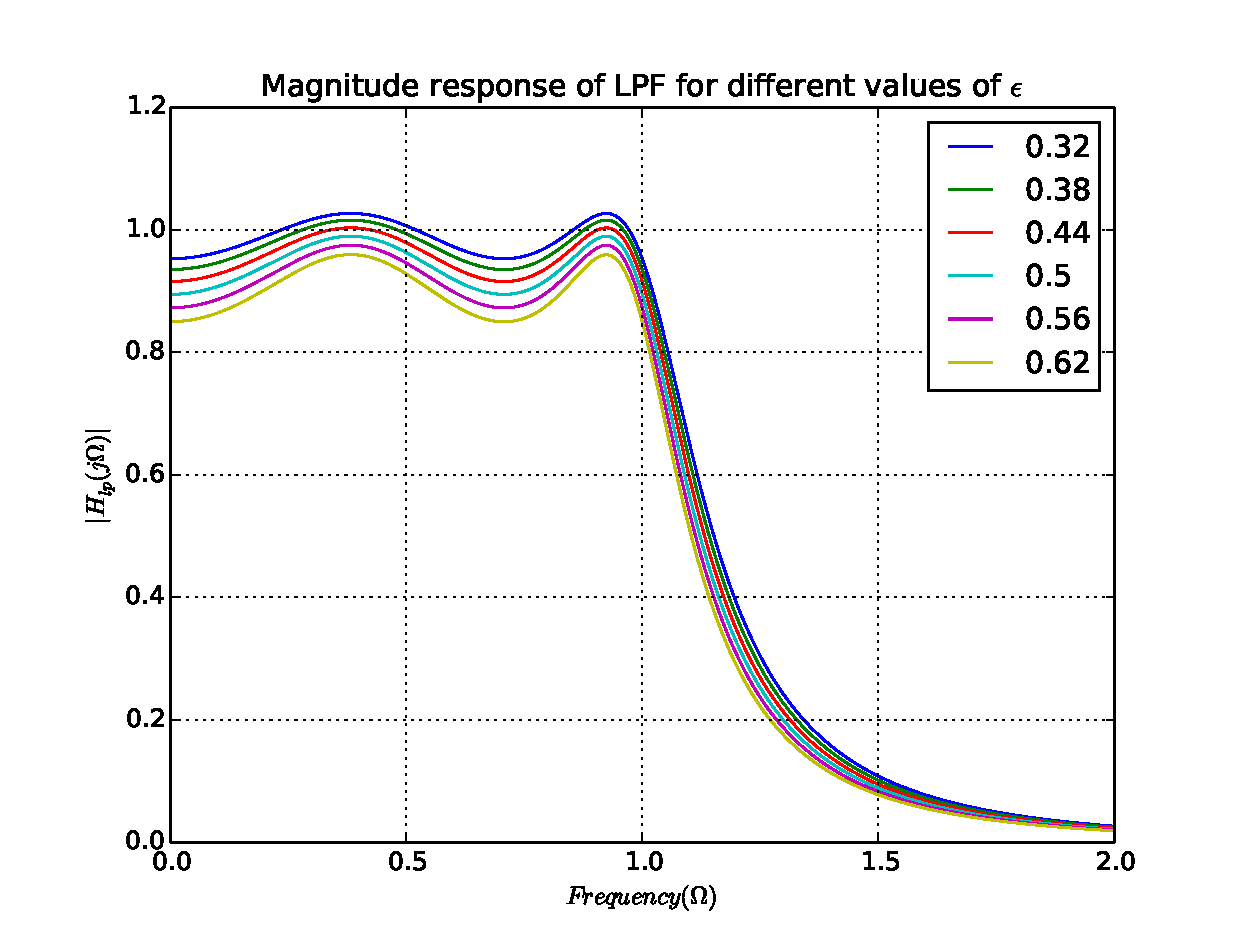
\includegraphics[width=\columnwidth]{./figs/lowpass.eps}
\caption{}
\label{fig:anaog_lpf}
\end{figure}
\begin{problem}
What value of $\varepsilon$ should be selected?
\end{problem}
\solution
There is a trade-off between passband and stopband frequencies. So select the $\varepsilon$ value which satisfies only passband frequency.
For the above example we assume $\varepsilon$=0.6197
\section{IIR Band Pass Analog Filter}
\begin{problem}
Obtain the band pass filter from low pass filter in \eqref{eq:bp_lp1}
\end{problem}
\solution

The analog band pass filter can be obtained from analog low pass filter as
\begin{equation}
H_{BP}(s) = H_{LP}(s_L)|_{s_L=\frac{s^2+\Omega_0^2}{Bs}}
\end{equation}
\begin{problem}
Write a Python script for computing coefficients of analog BPF for $N=4, \varepsilon = 0.6197$ and plot the magnitude response.
\end{problem}
\solution
\lstinputlisting{./codes/ABPF_Coeff.py}
\begin{figure}
\centering
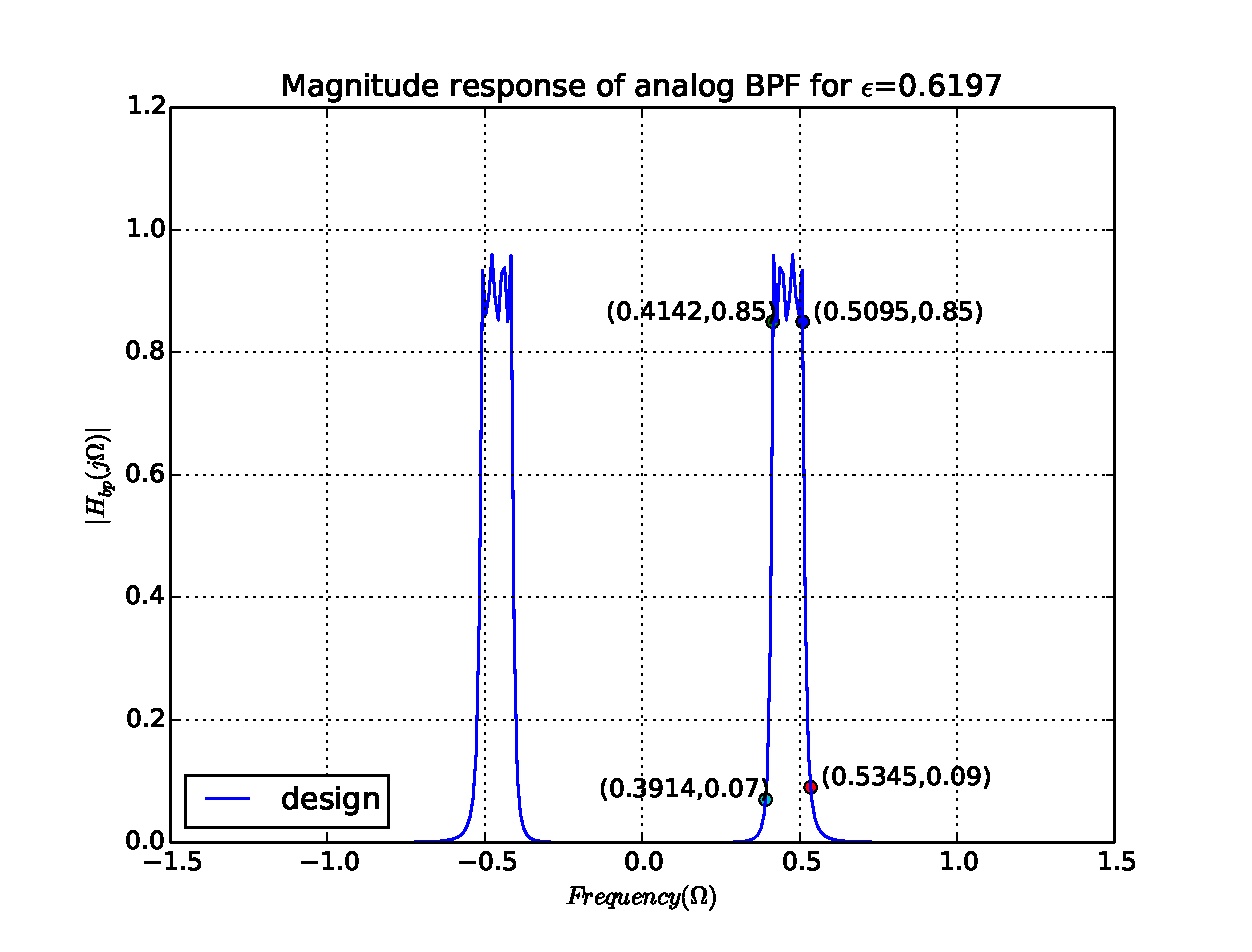
\includegraphics[width=\columnwidth]{./figs/analog_bpf.eps}
\caption{}
\label{fig:analog_bpf}
\end{figure}
\section{IIR Digital Band Pass Filter}
\begin{problem}
Obtain the IIR digital band pass filter from corresponding analog filter using Bilinear transformation.
\end{problem}
\solution
The IIR digital BPF can be obtained from the analog BPF as
\begin{equation}
H_{BP}(z) = H_{BP}(s)|_{s=\frac{1-z^{-1}}{1+z^{-1}}}
\end{equation}
%
\begin{problem}
Write a Python script for finding the digital BPF coefficinets from the analog BPF coefficients and plot the magnitude response of the digital BPF.
\end{problem}
\solution
\lstinputlisting{./codes/DBPF_Coeff.py}
\begin{figure}
\centering
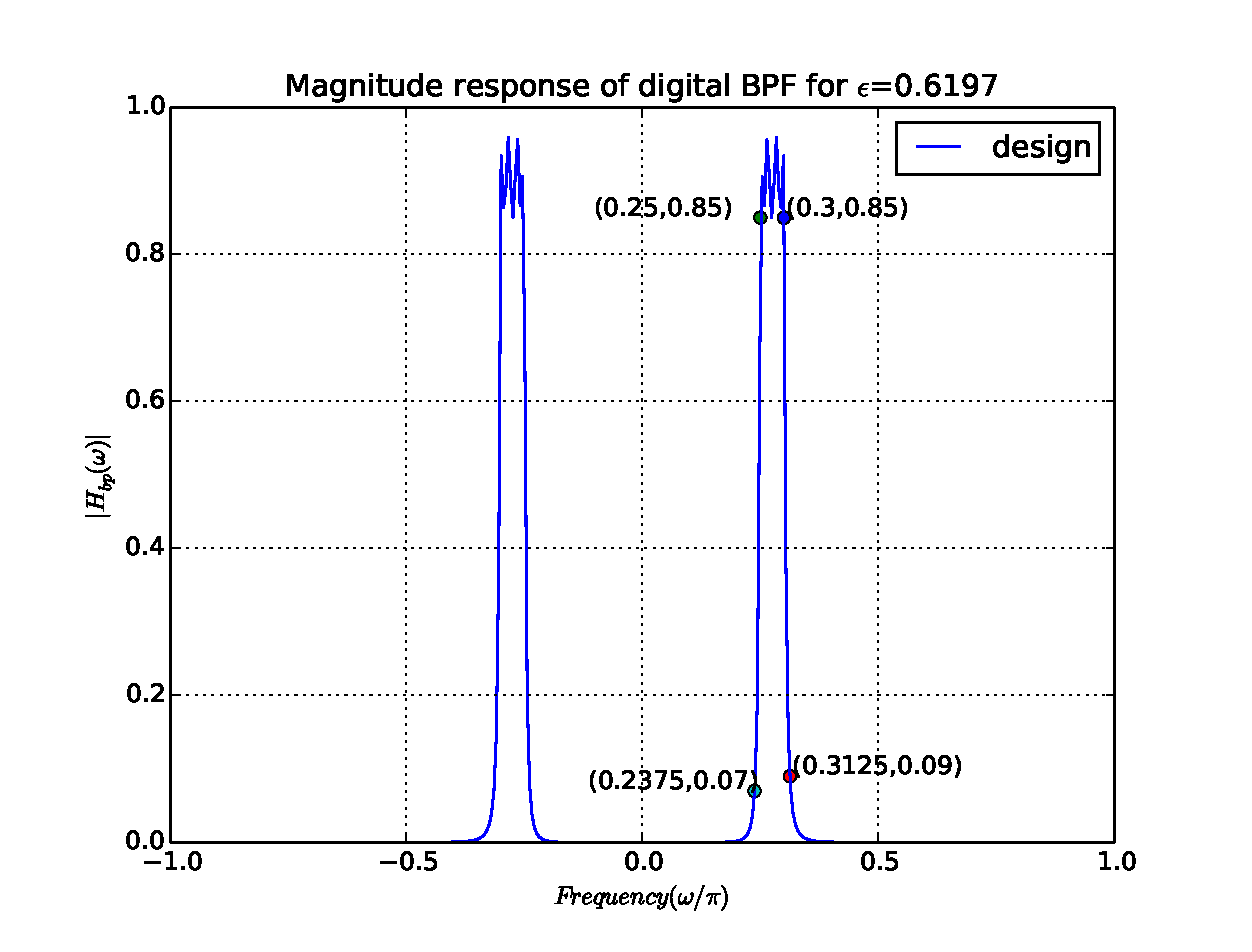
\includegraphics[width=\columnwidth]{./figs/digital_bpf.eps}
\caption{}
\label{fig:digital_bpf}
\end{figure}

\end{document}

